\documentclass[conference]{IEEEtran}
\IEEEoverridecommandlockouts
\usepackage{cite}
\usepackage{amsmath,amssymb,amsfonts}
\usepackage{algorithmic}
\usepackage{algorithm}
\usepackage{graphicx}
\usepackage{textcomp}
\usepackage{xcolor}
\usepackage{xurl}
\usepackage{booktabs}
\usepackage{stfloats}
\usepackage[
  letterpaper,
  left=19mm,
  textwidth=175mm,
  top=25mm,
  textheight=226mm,
  columnsep=8mm,
  noheadfoot
]{geometry}
\usepackage[font=small,labelsep=period]{caption}
\usepackage{titlesec}
% Use Times-like font (compatible with pdflatex and xelatex)
\usepackage{iftex}
\ifPDFTeX\else
  \usepackage{fontspec}
  \usepackage{xeCJK}
  \IfFontExistsTF{Times New Roman}{\setmainfont{Times New Roman}}{}
  \IfFontExistsTF{Noto Serif CJK TC}{\setCJKmainfont{Noto Serif CJK TC}}{}
\fi
\renewcommand{\ttdefault}{cmtt}
\setlength{\parindent}{1em}
\setlength{\footskip}{0pt}
\setlength{\columnsep}{8mm}
\setlength{\emergencystretch}{2em}
\def\IEEEtitletopspaceextra{8mm}
\renewcommand{\thesection}{\arabic{section}}
\renewcommand{\thesubsection}{\thesection.\arabic{subsection}}
\renewcommand{\thesubsubsection}{\thesubsection.\arabic{subsubsection}}
\AtBeginDocument{%
  \renewcommand{\thefigure}{\arabic{figure}}%
  \renewcommand{\thetable}{\arabic{table}}%
}
\DeclareCaptionLabelFormat{cvgipfig}{Fig. #2}
\DeclareCaptionLabelFormat{cvgiptable}{Table #2}
\captionsetup[figure]{labelformat=cvgipfig,justification=centering}
\captionsetup[table]{labelformat=cvgiptable,justification=centering}
\titleformat{\section}
  {\centering\normalfont\normalsize\bfseries}
  {\thesection.}{0.5em}{\MakeUppercase}
\titlespacing*{\section}{0pt}{1.0\baselineskip}{1.0\baselineskip}
\titleformat{\subsection}
  {\normalfont\normalsize\bfseries}
  {\thesubsection.}{0.5em}{}
\titlespacing*{\subsection}{0pt}{0.8\baselineskip}{0.4\baselineskip}
\titleformat{\subsubsection}
  {\normalfont\normalsize\itshape}
  {\thesubsubsection.}{0.5em}{}
\titlespacing*{\subsubsection}{0pt}{0.6\baselineskip}{0.3\baselineskip}
\newcommand{\algorithmicsymbols}{\textbf{Symbols:}}
\newcommand{\SYMBOLS}{\item[\algorithmicsymbols]}

\def\BibTeX{{\rm B\kern-.05em{\sc i\kern-.025em b}\kern-.08em
    T\kern-.1667em\lower.7ex\hbox{E}\kern-.125emX}}
\begin{document}

\title{\fontsize{14}{16}\selectfont\bfseries Feature-Guided Domain Selection for\\ High-Resolution Fractal Image Compression}

\author{
\IEEEauthorblockN{\textsuperscript{1,*}Zhen-Rong Wu and \textsuperscript{1}Liang-Yun Ko}
\IEEEauthorblockA{\textsuperscript{1}Department of Computer Science and Information Engineering,\\
National Taiwan Normal University, Taipei City, Taiwan,\\
E-mail: 41247012S@ntnu.edu.tw}
}

\maketitle

\begin{center}
    \textbf{ABSTRACT}
\end{center}
\noindent
Fractal Image Compression (FIC) provides fast, resolution-independent decoding, but high-resolution encoding remains expensive because each range block must search a large domain pool. This paper proposes Feature-Guided Domain Selection (FGDS), which shifts the heuristic from per-block optimization to domain-block selection. Each block is represented by an 8-dimensional, isometry-robust descriptor, and a KD-Tree retrieves the most similar domain candidates for a small exhaustive search. A Genetic Algorithm learns transferable feature weights from one held-out image. On ten \mbox{$1024\times1024$} grayscale images, the final FGDS+GA setting at \mbox{$K\!=\!80$} improves reconstruction PSNR over PSO by an average of 2.39~dB, reduces candidate-pool construction from 179.6~s to 0.13~s, and remains about twice as fast when preprocessing is included. A random-pool control confirms that the gain comes from feature-guided selection rather than search-space reduction alone.

\vspace{0.5\baselineskip}
\noindent
\textbf{Keywords:} Fractal image compression, feature-guided search, domain block selection, KD-Tree, genetic algorithm

\vspace{4mm}

%% ================================================================
\section{Introduction}
%% ================================================================

Fractal Image Compression (FIC) encodes an image as a set of contractive affine maps between image regions, exploiting self-affine redundancy to achieve compact, resolution-independent representations~\cite{Barnsley1985, FICOriginal}. Decoding is fast, iterating the stored maps from any starting image converges to a fixed-point reconstruction. Encoding, however, is the opposite. For every non-overlapping range block, the encoder must find, among all domain blocks and all eight geometric isometries, the transformation that minimizes reconstruction error. This search grows quadratically with image resolution and is the dominant cost of FIC.

A long-standing line of work replaces the exhaustive search with metaheuristics. Muruganandham and Wahida Banu~\cite{PSOFIC} applied Particle Swarm Optimization (PSO) to reduce encoding time, and genetic algorithms~\cite{wu2007schema, wu2006spatial, mitra1998technique} have been explored in the same spirit, drawing on the continuing development of swarm optimization~\cite{li2022pyramid}. These methods treat the domain index and isometry of each range block as the variables to be optimized, and search that space with a population of candidate~solutions.

We began by replicating this strategy on high-resolution (\mbox{$1024\times1024$})~images, where its limitations become clear. At this scale a single range block has \mbox{$P\!\times\!8 \approx 5.2\times10^5$}~domain--isometry candidates. A PSO swarm of 40~particles therefore inspects well under \mbox{$0.1\%$} of the space at initialization, and because the FIC objective over domain indices is highly non-smooth---spatially adjacent domains can have completely different content---the swarm has no reliable direction to follow and often converges to solutions far from the optimum. Adding memetic local search~\cite{moscato1989evolution} improves quality but cannot fully repair this: if the swarm settles in the wrong region of the pool, refining its neighborhood has limited value.

These findings suggest a different diagnosis. The difficulty is not that the optimizer is weak; it is that \emph{the search space handed to the optimizer is poorly chosen}. All domain-matching metaheuristics search indiscriminately over the full pool, spending most of their budget on structurally dissimilar blocks that can never yield a good match. That block matching can be accelerated by exploiting block structure is itself classical: Fisher pruned the pool by sorting blocks into a few discrete \emph{classes}~\cite{compression1995fractal}, and Saupe recast exhaustive matching as multi-dimensional nearest-neighbor search in an analytically derived feature space~\cite{saupe1995accelerating}. Our goal is not to reinvent feature-space matching, but to bring this structural view to the \emph{metaheuristic} formulation, which has continued to search the unstructured pool directly. The question we pursue is therefore not how to search the pool better, but whether the pool itself should be built differently.

The key design decision in this work is therefore to \textbf{move the heuristic from block \emph{matching} to block \emph{selection}}. Instead of optimizing which domain matches each range block, a fast, structure-aware heuristic is used to \emph{select} a small, high-quality candidate pool of domains per range block, which is then searched to optimality. This method is referred to as \textbf{Feature-Guided Domain Selection (FGDS)}. Concretely, FGDS (i)~computes an 8-dimensional descriptor designed to be robust to the eight FIC isometries, (ii)~uses a KD-Tree to retrieve the \mbox{$K$}~nearest domains for each range block in a learned weighted feature space, and (iii)~exhaustively evaluates the \mbox{$K\!\times\!8$}~candidates in that pool.

The main contributions of this paper are:
\begin{enumerate}
    \item \textbf{A reframing of the metaheuristic FIC problem} from per-block domain \emph{matching} to domain-block \emph{selection}, supported by an ablation showing that, once a feature-guided pool exists, exhaustive search dominates the inner PSO---so the optimizer can be removed entirely.
    \item \textbf{FGDS}, an 8-dimensional isometry-robust descriptor plus KD-Tree nearest-neighbor selection, which cuts candidate-pool construction from 179.6~s to 0.13~s (about a 1370-fold speedup) and reduces the per-range search space by a factor of over 800 at \mbox{$K\!=\!80$}.
    \item \textbf{A GA-based feature-weight learner} that discovers, offline on a single held-out image, the relative importance of each feature dimension and transfers it to unseen images, motivated by the structure of the FIC affine~model.
    \item \textbf{A controlled study on ten~high-resolution~images}, including a random-pool control and a \mbox{$K$-sensitivity} sweep, with Wilcoxon signed-rank significance (\mbox{$n = 10$}), establishing that the feature-guided pool---not the inner optimizer---is the source of the improvement.
\end{enumerate}


%% ================================================================
%% SECTION 2: RELATED WORK / BACKGROUND
%% ================================================================
\section{Background and Related Work}

\subsection{Fractal Image Compression}

FIC originates from the theory of Iterated Function Systems (IFS)~\cite{Barnsley1985}, whose Collage Theorem and Contractive Mapping Fixed-Point Theorem justify representing an image by contractive self-maps~\cite{barnsley1988better}. Jacquin~\cite{FICOriginal, 241507} turned this into a practical block-based coder.

A grayscale image of size \mbox{$N\times N$} is partitioned into a range pool~\mbox{$\mathcal{R}$} of \mbox{$M=(N/L)^2$} non-overlapping \mbox{$L\times L$} range blocks and a domain pool~\mbox{$\mathcal{D}$} of \mbox{$P=(\lfloor(N-2L)/\delta\rfloor+1)^2$} overlapping \mbox{$2L\times2L$} domain blocks taken with stride~\mbox{$\delta$}. Each domain block is downsampled to \mbox{$L\times L$} by \mbox{$2\times2$} average pooling. For a range block~\mbox{$v$} and a domain block~\mbox{$u$}, the encoder seeks a contractive affine map combining one of eight Dihedral isometries~\mbox{$T_k$} (\mbox{$k\in\{0,\dots,7\}$}) with a contrast~\mbox{$s$} and brightness~\mbox{$o$}:
\begin{equation}
    \hat{v} = s\cdot T_k(\mathrm{downsample}(u)) + o.
    \label{eq:affine}
\end{equation}
For a fixed \mbox{$(u,k)$}, the parameters \mbox{$s$} and \mbox{$o$} that minimize the mean squared error (MSE),
\begin{equation}
    \mathrm{MSE}(v,\hat{v}) = \frac{1}{L^2}\sum_{i,j}\bigl(v(i,j)-\hat{v}(i,j)\bigr)^2,
    \label{eq:mse}
\end{equation}
are given by the closed-form least-squares solution:
\begin{equation}
    s = \frac{L^2\sum v u_k - (\sum v)(\sum u_k)}{L^2\sum u_k^2 - (\sum u_k)^2},
    \quad
    o = \frac{\sum v - s\sum u_k}{L^2},
    \label{eq:so}
\end{equation}
where \mbox{$u_k=T_k(\mathrm{downsample}(u))$}. The best isometry is
\mbox{$k^*=\arg\min_k \mathrm{MSE}(v,\,s_k u_k+o_k)$}, and contractivity \mbox{$|s|<1$} is enforced for decode     convergence. One evaluation of (\ref{eq:mse})--(\ref{eq:so}) for a single \mbox{$(u,k)$} pair is defined as a \emph{Fitness Function Evaluation (FFE)}; it serves as the unit of search cost shared by all compared methods.

Quality is reported as reconstruction Peak Signal-to-Noise Ratio (PSNR), computed between the original image and the image obtained after 20~decoding iterations from the selected affine maps; this isolates the effect of the search strategy before coefficient quantization. Where tables also list an encoder-side MSE, it is the average block-matching MSE of the selected maps---a direct measure of search quality---whereas the headline PSNR always refers to the decoded~reconstruction.

\paragraph*{Compression ratio} Each code stores a domain index, an isometry index \mbox{$k^*$}, and quantized \mbox{$s,o$}, costing $b_{\text{code}}=\lceil\log_2 P\rceil + 3 + b_s + b_o$~bits. With \mbox{$N\!=\!1024$}, \mbox{$L\!=\!4$}, \mbox{$\delta\!=\!4$} (so \mbox{$P=65{,}025$}), and \mbox{$b_s\!=\!8$}, \mbox{$b_o\!=\!12$}, this gives \mbox{$b_{\text{code}}=39$}~bits and \mbox{$\mathrm{CR}=N^2\!\cdot\!8/(M\,b_{\text{code}})\approx3.28{:}1$}. Because all methods use identical partitioning and code fields, CR is fixed throughout, and the comparison reduces to reconstruction quality and time under a common representation.

\subsection{Acceleration and metaheuristic FIC}

Exhaustive FIC evaluates all \mbox{$P\!\times\!8$}~candidates per range block, and two largely separate lines reduce this cost. The first exploits block \emph{structure}: quad-tree partitioning~\cite{compression1995fractal}, tree-structured codebook classification~\cite{478245, hurtgen1993fast}, parallel hardware~\cite{hufnagl2000algorithms, vidya2000architecture}, and---closest to our descriptor---Saupe's reformulation of block matching as multi-dimensional nearest-neighbor search~\cite{saupe1995accelerating}; recent encoders continue this structural line with block-feature pruning and adaptive partitioning~\cite{li2024centroid, li2025partition}. The second treats \mbox{$(d,k)$} as decision variables and applies a metaheuristic optimizer: PSO~\cite{PSOFIC, PSOOriginal, eberhart1995new} or genetic algorithms~\cite{wu2007schema, wu2006spatial, mitra1998technique}, building on broader swarm-optimization advances~\cite{li2022pyramid}. These lines developed independently, and the metaheuristic work still searches the full, unstructured pool. We connect them: rather than proposing another optimizer or rederiving Saupe's exact nearest-neighbor equivalence, we use feature-space \emph{selection} to construct the search space, then show through controlled ablation and a random-pool control that the metaheuristic \emph{matcher} inside that space is unnecessary. A metaheuristic does remain useful---but one level up, as a GA that designs the feature space itself.


%% ================================================================
%% SECTION 3: BASELINE METHODS AND THE PATH TO FGDS
%% ================================================================
\section{From PSO to Feature-Guided Selection}
\label{sec:baselines}

This section describes the compared baseline methods in the logical order of the development that led to FGDS. All share the fitness function of (\ref{eq:mse})--(\ref{eq:so}) and the same FFE accounting, so differences reflect only \emph{search strategy}.

\subsection{Standard PSO (baseline)}
Following~\cite{PSOFIC}, each particle is a continuous vector \mbox{$\mathbf{X}_j=[d_j,k_j]$} decoded to a (domain index, isometry) pair by rounding and clamping. The swarm updates
\begin{align}
    \mathbf{V}_j(t\!+\!1) & = \omega\mathbf{V}_j(t) + c_1 r_1(\mathbf{P}_{\text{best},j}\!-\!\mathbf{X}_j) \notag\\
    &\quad + c_2 r_2(\mathbf{G}_{\text{best}}\!-\!\mathbf{X}_j), \\
    \mathbf{X}_j(t\!+\!1) & = \mathbf{X}_j(t) + \mathbf{V}_j(t\!+\!1),
\end{align}
with swarm size \mbox{$N_p\!=\!40$}, inertia \mbox{$\omega\!=\!0.9$}, acceleration coefficients \mbox{$c_1\!=\!c_2\!=\!2.0$}, uniform random \mbox{$r_1,r_2\in[0,1]$}, and velocity clamped to \mbox{$\pm v_{\max}$}. The search domain is \mbox{$[0,P\!-\!1]\times[0,7]$}.

\subsection{Memetic PSO}
Memetic PSO applies deterministic local search after periodic PSO updates. To limit overhead, LS is applied only to the top 20\%~of particles ranked by fitness, followed by one terminal LS pass on the final global best. For one range block, write a candidate as \mbox{$x=(d,k)$}, where \mbox{$d$} indexes a domain block and \mbox{$k\in\mathcal{I}=\{0,\ldots,7\}$} is an isometry. Let \mbox{$f(d,k)$} denote the resulting block-wise MSE after fitting \mbox{$s,o$}; lower is better, so LS accepts only non-worsening moves. \textbf{Isometry-LS} fixes \mbox{$d$} and tests candidate isometries \mbox{$k'\in\mathcal{I}$}:
\begin{equation}
    k^*=\arg\min_{k'\in\mathcal{I}} f(d,k').
    \label{eq:isometry_ls}
\end{equation}
Since \mbox{$(d,k)$} is already evaluated, only the other seven isometries are new (\mbox{$\le7$}~FFEs). \textbf{Spatial-LS} then fixes \mbox{$k^*$} and searches the grid-neighbors \mbox{$\mathcal{N}_8(d)$} of \mbox{$d$}:
\begin{equation}
    d^*=\arg\min_{d'\in\{d\}\cup\mathcal{N}_8(d)} f(d',k^*),
    \label{eq:spatial_ls}
\end{equation}
again at most eight new evaluations (fewer on boundaries). All LS evaluations count against the FFE~budget. This is the first finding: local search reliably raises PSNR but costs time~(Section~\ref{sec:exp1}).

\subsection{Feature-Guided PSO (FG-PSO)}
This observation motivated restricting the search space of the PSO. FG-PSO first builds, for each range block, a feature-guided candidate pool of \mbox{$K$}~domains (Section~\ref{sec:proposed}), then runs the same memetic PSO inside the reduced subspace \mbox{$[0,K\!-\!1]\times[0,7]$}~rather than the full pool. Shrinking the space from approximately \mbox{$5\times10^5$} to \mbox{$K\!\times\!8$}~candidates lets a small swarm cover a meaningful fraction of it, and FG-PSO outperforms both baseline PSO variants. This stage is kept as a development baseline because it isolates the effect of feature-guided pool construction before the optimizer is removed.

\subsection{The ablation that removed the optimizer}
FG-PSO raises an obvious question: once the pool is reduced to only \mbox{$K\!=\!40$}~domains (\mbox{$320$}~candidates), does the metaheuristic search still buy anything over a complete scan? Replacing the inner PSO with a plain exhaustive scan of all \mbox{$K\!\times\!8$}~candidates---\emph{feature-guided exhaustive search}, the basis of FGDS---answers it: this variant matches or outperforms FG-PSO at higher PSNR with fewer FFEs (\mbox{$320$}~vs.\ the 800~budget), zero stochastic variance, and shorter runtime (Section~\ref{sec:exp1}). Within a few-hundred-candidate space a complete scan is simply more effective, so the metaheuristic matcher can be discarded and the remaining value placed where it belongs: in candidate-pool selection, the focus of the rest of this paper.


%% ================================================================
\section{Proposed Method: Feature-Guided Domain Selection}
\label{sec:proposed}
%% ================================================================

FGDS replaces metaheuristic block matching with feature-guided block selection followed by a small exhaustive search. The final pipeline is
\[
    \text{Block}\to\text{Feature Extraction}\to\text{Weighted Feature Space}
\]
\[
    \to\text{KD-Tree NN}\to\text{Candidate Pool}\to\text{Exhaustive Search}.
\]
An offline Genetic Algorithm (Section~\ref{sec:ga_weights}) learns the feature weights once and is not part of per-image encoding.

\begin{algorithm}[t]
    \caption{FGDS Encoding Pipeline}
    \label{alg:fgds}
    \begin{algorithmic}[1]
        \REQUIRE Image \mbox{$I$} (\mbox{$N\times N$}); range size \mbox{$L$}; stride \mbox{$\delta$}; pool size \mbox{$K$}; weights \mbox{$\mathbf{w}\in\mathbb{R}^8$}
        \SYMBOLS \mbox{$\mathbf f_R,\mathbf f_D$}: range/domain feature matrices; \mbox{$\boldsymbol\mu_D,\boldsymbol\sigma_D$}: domain-feature mean/std.; \mbox{$\hat{\mathbf f}$}: normalized feature; \mbox{$\hat{\mathbf f}_D,\hat{\mathbf f}_{R,i}$}: weighted domain features and the \mbox{$i$}-th weighted range feature
        \ENSURE Fractal codes \mbox{$\mathcal{C}$}
        \STATE \textbf{// Stage 1: Feature Extraction}
        \STATE \mbox{$\mathbf{f}_R\leftarrow\textsc{ExtractFeatures}(\text{range blocks})$} \COMMENT{\mbox{$(M,8)$}}
        \STATE \mbox{$\mathbf{f}_D\leftarrow\textsc{ExtractFeatures}(\text{domain blocks})$} \COMMENT{\mbox{$(P,8)$}}
        \STATE \mbox{$z$}-score normalize \mbox{$\mathbf{f}_R,\mathbf{f}_D$} using \mbox{$(\boldsymbol{\mu}_D,\boldsymbol{\sigma}_D)$}
        \STATE Apply weights: \mbox{$\hat{\mathbf{f}}\leftarrow\hat{\mathbf{f}}\odot\mathbf{w}$} \COMMENT{element-wise}
        \STATE \textbf{// Stage 2: KD-Tree Candidate Pool}
        \STATE Build KD-Tree \mbox{$\mathcal{T}$} from \mbox{$\hat{\mathbf{f}}_D$}
        \FOR{each range block \mbox{$v_i$}}
        \STATE \mbox{$\mathcal{P}_i\leftarrow\mathcal{T}.\text{query}(\hat{\mathbf{f}}_{R,i},K)$} \COMMENT{top-\mbox{$K$} neighbors}
        \ENDFOR
        \STATE \textbf{// Stage 3: Exhaustive Search in Reduced Space}
        \FOR{each range block \mbox{$v_i$}}
        \STATE \mbox{$(d^*,k^*,s^*,o^*)\leftarrow$}
        \STATE \hspace{\algorithmicindent}\mbox{$\arg\min_{j\in\mathcal{P}_i,k}\mathrm{MSE}(v_i, sT_k(u_j)\!+\!o)$}
        \STATE \mbox{$\mathcal{C}_i\leftarrow(d^*,k^*,s^*,o^*)$}
        \ENDFOR
        \RETURN \mbox{$\mathcal{C}$}
    \end{algorithmic}
\end{algorithm}

\subsection{Stage 1: Isometry-robust features}
The descriptor must (R1) discriminate structurally dissimilar blocks and (R2) be robust to the eight Dihedral isometries, since a domain under any of these transforms is the same candidate and the isometry is searched separately in Stage~3. For a block \mbox{$b$} of size \mbox{$L\times L$}, the feature vector is defined as
\begin{equation}
    \mathbf{f}(b)=\bigl[\mu,\ \sigma,\ \bar g_h,\ \bar g_v,\ \hat q_1,\ \hat q_2,\ \hat q_3,\ \hat q_4\bigr]\in\mathbb{R}^8.
    \label{eq:features}
\end{equation}
Here \mbox{$\mu$} and \mbox{$\sigma$} are the block mean and standard deviation, both exactly invariant to the eight isometries. \mbox{$\bar g_h=\mathrm{mean}|b(i,j\!+\!1)\!-\!b(i,j)|$} and \mbox{$\bar g_v=\mathrm{mean}|b(i\!+\!1,j)\!-\!b(i,j)|$} are mean gradient magnitudes capturing texture; they are invariant under horizontal and vertical flips and swap under \mbox{$90^\circ$} rotation, so they are treated as quasi-invariant directional texture cues rather than strict invariants. The \mbox{$\hat q_1\!\le\!\dots\!\le\!\hat q_4$} are the four quadrant means \emph{sorted ascending}: rotations and reflections only permute quadrants, so sorting makes them fully isometry-invariant. Each feature costs \mbox{$O(L^2)$}.

Features are \mbox{$z$}-score normalized with domain-pool statistics, \mbox{$\hat{\mathbf f}=(\mathbf f-\boldsymbol\mu_D)/(\boldsymbol\sigma_D+10^{-8})$}, so every dimension contributes comparably to Euclidean distance before weighting.

\subsection{Stage 2: KD-Tree candidate selection}
For each range block \mbox{$v_i$}, the \mbox{$K$} nearest domain blocks in the weighted feature space are determined by
\begin{equation}
    \mathcal{P}_i=\underset{|S|=K}{\arg\min}\sum_{j\in S}\bigl\|\mathbf w\odot(\hat{\mathbf f}_{R,i}-\hat{\mathbf f}_{D,j})\bigr\|^2 .
    \label{eq:knn}
\end{equation}
Pre-multiplying both feature sets by \mbox{$\mathbf w$} turns this into plain Euclidean nearest-neighbor search, so a standard KD-Tree~\cite{bentley1975multidimensional} applies. Over the \mbox{$F\!=\!8$}~feature dimensions, a naive pairwise scan costs \mbox{$O(MPF)$} (here approximately 180~s), whereas the KD-Tree costs \mbox{$O(PF\log P)$}~to build and \mbox{$O(MK\log P)$}~to query, completing in under 0.5~s in practice. With \mbox{$K\!=\!80$}~the per-range space shrinks from \mbox{$P\!\times\!8=520{,}200$} to \mbox{$640$}~candidates, a reduction of over 800-fold. Since the descriptor dimension is only \mbox{$F\!=\!8$}, KD-Tree search remains effective in our setting, as confirmed by the measured candidate-selection~time.

\subsection{Stage 3: Exhaustive search in the pool}
Within \mbox{$\mathcal{P}_i$}, all \mbox{$K\!\times\!8$}~domain--isometry pairs are evaluated via (\ref{eq:mse})--(\ref{eq:so}) to select the minimum-MSE candidate satisfying \mbox{$|s|<1$}. Unlike PSO, which rounds continuous positions to discrete indices and may skip candidates, this scan is exact within the pool. With \mbox{$K\!=\!80$}~it costs \mbox{$640$}~FFEs per block---fewer than the budgets given to the PSO baselines---yet it is guaranteed optimal over the selected domains.


\subsection{Learning feature weights with a Genetic Algorithm}
\label{sec:ga_weights}

Equal weighting (\mbox{$\mathbf w=\mathbf 1$}) assumes all eight dimensions matter equally for pool quality, which is not true: the dimensions play different roles in the affine match of (\ref{eq:so}). Therefore, the weight vector \mbox{$\mathbf w\in\mathbb{R}^8_{>0}$} is learned using a Genetic Algorithm run \emph{once, offline}, on a single training image disjoint from the test set, and applied to all test images at zero extra encoding cost. This is a deliberately different use of a metaheuristic from the discarded PSO matcher: GA optimizes the \emph{design of the feature space}, not the per-block search.

\paragraph*{Fitness} An individual is a weight vector \mbox{$\mathbf w$}. Fitness is the negative average MSE obtained by running weighted KD-Tree selection and exhaustive search on a random 2\% sample of range blocks (\mbox{$\approx$}1{,}300 blocks for \mbox{$1024^2$}). Raw features and isometry tables are precomputed, so each evaluation only re-weights features, rebuilds the tree, and scans the sample.

\paragraph*{Settings and result} We use tournament selection, BLX-\mbox{$\alpha$} crossover~\cite{eshelman1993real}, Gaussian mutation, and two elites, with \mbox{$N_{\text{pop}}\!=\!16$}, \mbox{$G\!=\!10$}, \mbox{$\rho\!=\!0.02$}, and \mbox{$K\!=\!80$}. On held-out image~0003, sampled MSE improves from 72.82 to 71.77 and converges to
\begin{equation}
    \mathbf{w}^* = [\,0.18,\ 1.36,\ 0.97,\ 0.96,\ 1.29,\ 1.04,\ 1.00,\ 0.75\,]
    \label{eq:learned_w}
\end{equation}
for \mbox{$[\mu,\sigma,\bar g_h,\bar g_v,\hat q_1,\hat q_2,\hat q_3,\hat q_4]$}. The learned vector is consistent with the model-structure argument below: the mean \mbox{$\mu$} receives by far the smallest weight (0.18) and the standard deviation \mbox{$\sigma$} the largest (1.36)---a 7.6-fold difference---matching the ``down-weight \mbox{$\mu$}---up-weight \mbox{$\sigma$}'' prediction. The gradient and quadrant features stay near 1.0, consistent with their secondary role at \mbox{$L\!=\!4.$}

\paragraph*{Why one training image generalizes}
\label{sec:generalize}
The weights reflect the affine model rather than image content. In (\ref{eq:so}), mean mismatch is largely absorbed by the offset \mbox{$o$}, whereas standard-deviation mismatch affects the contrast \mbox{$s$} and can violate contractivity. Thus the learned low \mbox{$w_\mu$} and high \mbox{$w_\sigma$} are model-driven, and empirically improve PSNR on all ten unseen images (Section~\ref{sec:exp2}).

\subsection{Computational complexity}
\begin{table}[t]
    \centering
    \caption{Per-range search cost and preprocessing. Symbols: \mbox{$P$}~domain blocks, \mbox{$M$}~range blocks, \mbox{$L$}~range size, \mbox{$K$}~pool size, \mbox{$F\!=\!8$}~feature dimensions, \mbox{$B$}~per-block FFE budget.}
    \label{tab:complexity}
    \small
    \setlength{\tabcolsep}{2pt}
    \begin{tabular}{lll}
        \toprule
        \textbf{Method}         & \textbf{Per-range cost} & \textbf{Preprocessing}                                                                        \\
        \midrule
        Full search             & \mbox{$O(P\cdot 8)$}    & \mbox{$O(P L^2)$}                                                                             \\
        PSO (budget \mbox{$B$}) & \mbox{$O(B)$}           & \mbox{$O(P L^2)$}                                                                             \\
        FGDS (proposed)         & \mbox{$O(K\cdot 8)$}    & $\begin{array}{@{}l@{}}O((M+P)L^2 + PF\log P\\{}+ MK\log P)\end{array}$ \\
        \bottomrule
    \end{tabular}
\end{table}
Table~\ref{tab:complexity} summarizes the costs. FGDS trades a sub-second KD-Tree preprocessing step for a per-range cost of only \mbox{$K\!\times\!8$}~FFEs. A full search at \mbox{$1024^2$} would require \mbox{$M\!P\!\times\!8\approx 3.4\times10^{10}$}~FFEs per image; FGDS at \mbox{$K\!=\!80$} uses \mbox{$M\!\times\!640\approx 4.2\times10^7$}, a reduction of over \mbox{$800\times$}, while the GA cost is one-time and offline.


%% ================================================================
\section{Experimental Setup}
\subsection{Hardware and implementation}
Experiments run on an AMD EPYC 7313P 16-core server with FreeBSD 15.0. All methods are implemented in Python/NumPy; FGDS uses SciPy's \texttt{KDTree}.

\subsection{Data}
The dataset consists of ten images from DIV2K~\cite{div2k}---0002, 0007, 0029, 0030, 0032, 0037, 0043, 0049, 0051, 0060---each resized to \mbox{$1024\times1024$} and converted to 8-bit grayscale. The GA training image (0003) is \emph{not} in the test set, so all reported GA results are on unseen images.

\subsection{FIC parameters}
\mbox{$L\!=\!4$}, \mbox{$2L\!=\!8$}, \mbox{$\delta\!=\!4$}, giving \mbox{$M=65{,}536$} range and \mbox{$P\!=\!65{,}025$} domain blocks. The stored code uses \mbox{$b_s=8$} and \mbox{$b_o=12$}, giving \mbox{$b_{\text{code}}=39$} bits and \mbox{$\mathrm{CR}\approx3.28{:}1$}; decoding uses 20~iterations.

\subsection{Budget and protocol}
The FFE budget is fixed at 800~per range block. This is generous for FGDS---at \mbox{$K\!=\!80$} it finishes in \mbox{$K\!\times\!8\!=\!640$}~FFEs and is flat thereafter---and is chosen so the convergence plots show, on a common axis, exactly when each method saturates. Stochastic methods (PSO, memetic PSO, FG-PSO) run 5~times per image with seeds \mbox{$\{42,\dots,46\}$}; FGDS is deterministic. Pairwise comparisons use the Wilcoxon signed-rank test~\cite{wilcoxon1945individual} over the \mbox{$n\!=\!10$}~images.

\subsection{Experiments}
The study is a single connected line of evidence, organized as four runs:
\textbf{(E1)} PSO vs.\ memetic PSO vs.\ FG-PSO vs.\ FGDS-exhaustive, all feature-based methods at \mbox{$K\!=\!40$}, establishing the optimizer-removal result;
\textbf{(E2)} the three FGDS variants---pairwise, KD-Tree, and KD-Tree+GA weights---at \mbox{$K\!=\!80$}, isolating the preprocessing speedup and the GA contribution;
\textbf{(E3)} a \mbox{$K$}-sensitivity sweep \mbox{$K\in\{5,10,20,40,80,160\}$} for KD-Tree FGDS, locating the best quality--time trade-off under the fixed FFE protocol;
\textbf{(E4)} a same-size random-pool control vs.\ FGDS, both at \mbox{$K\!=\!80$}, attributing the gain to feature-guided selection.
E1 fixes \mbox{$K\!=\!40$} because that was the pool size used by FG-PSO in the development ablation; the \mbox{$K$}-sweep of E3 then justifies adopting \mbox{$K\!=\!80$} for E2 and E4. E1 reports only the search-loop wall-clock time, excluding feature extraction and candidate-pool construction, in order to isolate the optimizer effect; E2 and E3 then separately report preprocessing and total time for the final FGDS variants.


%% ================================================================
\section{Results}
%% ================================================================

\subsection{E1: Optimizer vs.\ search-space quality}
\label{sec:exp1}

\begin{table*}[t]
    \centering
    \caption{E1: PSO baselines vs.\ FGDS (feature-guided exhaustive, \mbox{$K\!=\!40$}) on ten \mbox{$1024\times1024$}~images. Time reports the search-loop wall-clock time of a \emph{single} encode, excluding feature extraction and candidate-pool construction; for the stochastic methods both Time and PSNR are the mean over 5~runs (PSNR std \mbox{$\le 0.03$}~dB), not the cumulative cost of those runs. FGDS is deterministic. Best per image in bold.}
    \label{tab:results}
    \begin{tabular}{l rrrr rrrr}
        \toprule
                       & \multicolumn{2}{c}{\textbf{PSO}} & \multicolumn{2}{c}{\textbf{Memetic PSO}} & \multicolumn{2}{c}{\textbf{FG-PSO} (\mbox{$K\!=\!40$})} & \multicolumn{2}{c}{\textbf{FGDS} (\mbox{$K\!=\!40$})}                                                     \\
        \cmidrule(lr){2-3}\cmidrule(lr){4-5}\cmidrule(lr){6-7}\cmidrule(lr){8-9}
        \textbf{Image} & Time(s)                          & PSNR                                     & Time(s)                                                 & PSNR                                                  & Time(s) & PSNR  & Time(s)        & PSNR           \\
        \midrule
        0002           & 1432.1                           & 28.73                                    & 1299.3                                                  & 28.87                                                 & 1286.4  & 29.58 & \textbf{364.5} & \textbf{30.00} \\
        0007           & 1429.8                           & 26.32                                    & 1301.7                                                  & 26.45                                                 & 1289.1  & 27.14 & \textbf{363.8} & \textbf{27.58} \\
        0029           & 1441.3                           & 23.47                                    & 1301.2                                                  & 23.69                                                 & 1285.3  & 24.89 & \textbf{365.6} & \textbf{25.43} \\
        0030           & 1421.3                           & 30.52                                    & 1302.2                                                  & 30.84                                                 & 1284.8  & 31.71 & \textbf{358.5} & \textbf{32.26} \\
        0032           & 1412.5                           & 33.78                                    & 1308.4                                                  & 34.03                                                 & 1252.5  & 35.00 & \textbf{354.4} & \textbf{35.47} \\
        0037           & 1414.3                           & 32.17                                    & 1345.8                                                  & 32.65                                                 & 1250.6  & 34.07 & \textbf{354.5} & \textbf{34.66} \\
        0043           & 1412.0                           & 27.70                                    & 1343.8                                                  & 28.20                                                 & 1249.8  & 30.26 & \textbf{354.3} & \textbf{30.92} \\
        0049           & 1412.9                           & 29.96                                    & 1337.2                                                  & 30.12                                                 & 1249.7  & 31.23 & \textbf{354.8} & \textbf{31.71} \\
        0051           & 1411.1                           & 27.78                                    & 1302.2                                                  & 28.04                                                 & 1270.9  & 28.86 & \textbf{354.9} & \textbf{29.31} \\
        0060           & 1410.7                           & 28.31                                    & 1330.0                                                  & 28.60                                                 & 1268.7  & 29.99 & \textbf{354.8} & \textbf{30.68} \\
        \midrule
        \textbf{Avg}   & 1419.8                           & 28.87                                    & 1317.2                                                  & 29.15                                                 & 1268.8  & 30.27 & \textbf{358.0} & \textbf{30.80} \\
        \bottomrule
    \end{tabular}
\end{table*}

Table~\ref{tab:results} traces the full trail. Memetic PSO improves PSO on every image (+0.28~dB average) but adds cost. FG-PSO then gains +1.12~dB by searching a feature-guided pool, showing that \emph{search-space quality} is the missing factor. Replacing the inner PSO with exhaustive search over the same \mbox{$K\!=\!40$} pool---FGDS---adds another +0.53~dB with fewer FFEs (\mbox{$320$} vs.\ 800), no randomness, and much less time.

\textbf{Magnitude and speed.} FGDS exceeds PSO by 1.26--3.22~dB (mean~+1.93), memetic PSO by 1.13--2.72~dB (mean~+1.65), and FG-PSO by 0.42--0.69~dB (mean~+0.53), while averaging 358~s per image against 1420~s, 1317~s, and 1269~s, respectively. The time is for one encode per method; the saving comes from the compact \mbox{$320$}-FFE per-range search, and Section~\ref{sec:exp2} adds preprocessing time for the final \mbox{$K\!=\!80$} KD-Tree setting.

The decisive comparison is FG-PSO vs.\ FGDS: the same pool, with and without the inner PSO. FGDS wins on all ten images at fewer evaluations, so a complete scan is preferable once the candidate space is small. Figure~\ref{fig:conv_exp1} shows that the feature-guided methods are already 2--3~dB above the PSO baselines at the first recorded point, and FGDS saturates at \mbox{$K\!\times\!8=320$}~FFEs.

\begin{figure}[t]
    \centering
    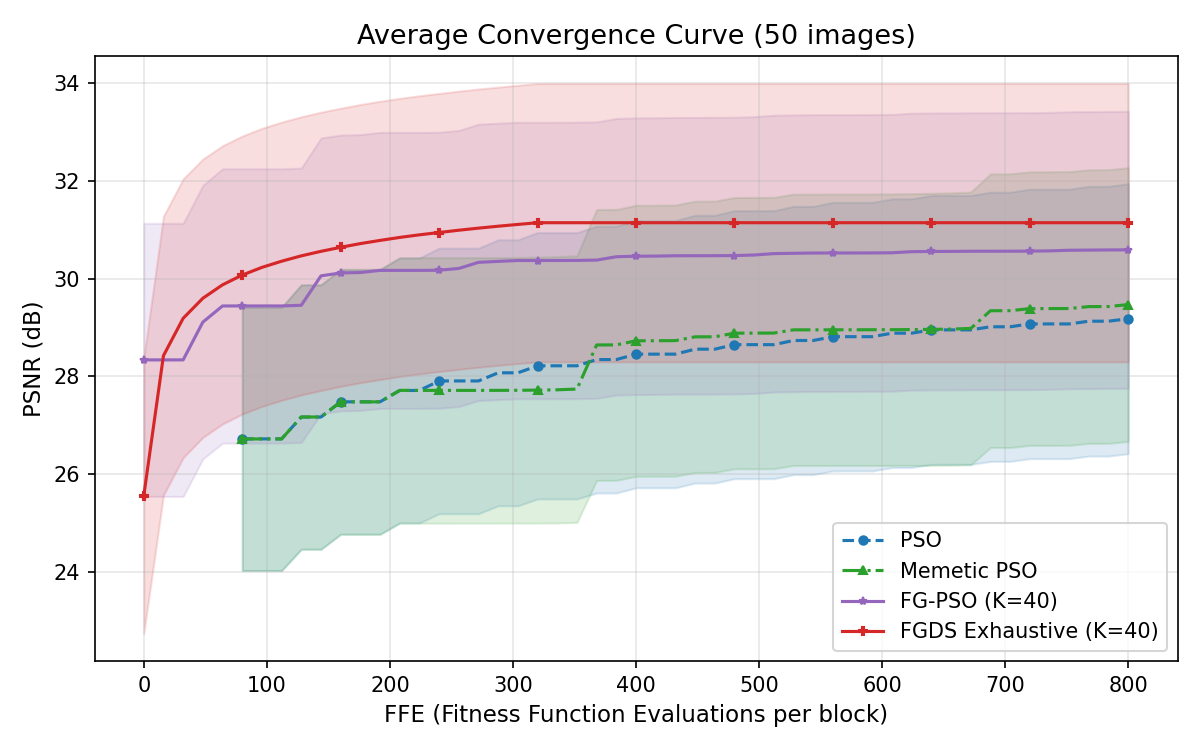
\includegraphics[width=\columnwidth]{images/convergence_average_exp1.png}
    \caption{E1 convergence averaged over the ten~images (5~runs each; \mbox{$\pm1\sigma$} bands). At the first recorded evaluation point, the feature-guided methods are already above the PSO baselines; FGDS saturates at 320~FFEs and remains the highest.}
    \label{fig:conv_exp1}
\end{figure}

\subsection{E2: KD-Tree acceleration and GA weights}
\label{sec:exp2}

\begin{table}[t]
    \centering
    \caption{E2: three FGDS variants at \mbox{$K\!=\!80$}, averaged over ten images. Times in seconds; CandSel = candidate selection. MSE is encoder-side block-matching MSE. PSNR/MSE for pairwise and KD-Tree are identical by construction.}
    \label{tab:exp2}
    \small
    \setlength{\tabcolsep}{2pt}
    \begin{tabular}{lrrrrr}
        \toprule
        \textbf{Variant} & \textbf{PSNR}  & \textbf{MSE} & \textbf{Feat.} & \textbf{Cand.} & \textbf{Enc.} \\
        \midrule
        Pairwise         & 31.21          & 56.27             & 7.20             & 179.57           & 697.80          \\
        KD-Tree          & 31.21          & 56.27             & 7.22             & \textbf{0.13}    & 692.81          \\
        KD-Tree + GA     & \textbf{31.26} & \textbf{55.60}    & 7.22             & 0.12             & 692.10          \\
        \bottomrule
    \end{tabular}
\end{table}

Two questions are answered in Table~\ref{tab:exp2}.

\textbf{Does the KD-Tree change results?} No. It returns the same nearest neighbors as the pairwise scan, so PSNR and encoder-side MSE are identical (31.21~dB, 56.27~MSE), while candidate selection falls from 179.6~s to 0.13~s. Feature extraction remains about 7.2~s.

\textbf{What does the GA add?} Learned weights raise PSNR on all ten images by +0.01~to~+0.09~dB (mean~+0.05~dB, 31.21\mbox{$\to$}31.26), reduce encoder-side MSE (56.27\mbox{$\to$}55.60), and add no per-image encoding cost. The gain is small but uniformly positive (Wilcoxon \mbox{$W^+\!=\!55$}, \mbox{$p\!<\!0.01$}) and matches Section~\ref{sec:generalize}: the held-out training image learns to down-weight the offset-absorbed mean and up-weight the contrast-driving standard deviation. Thus GA is not the main source of improvement; it only learns transferable feature importance.

Figure~\ref{fig:conv_0030} shows the three variants on image 0030; the curves are visually indistinguishable, reflecting the near-identical PSNR, with the GA curve marginally on top.

\begin{figure}[t]
    \centering
    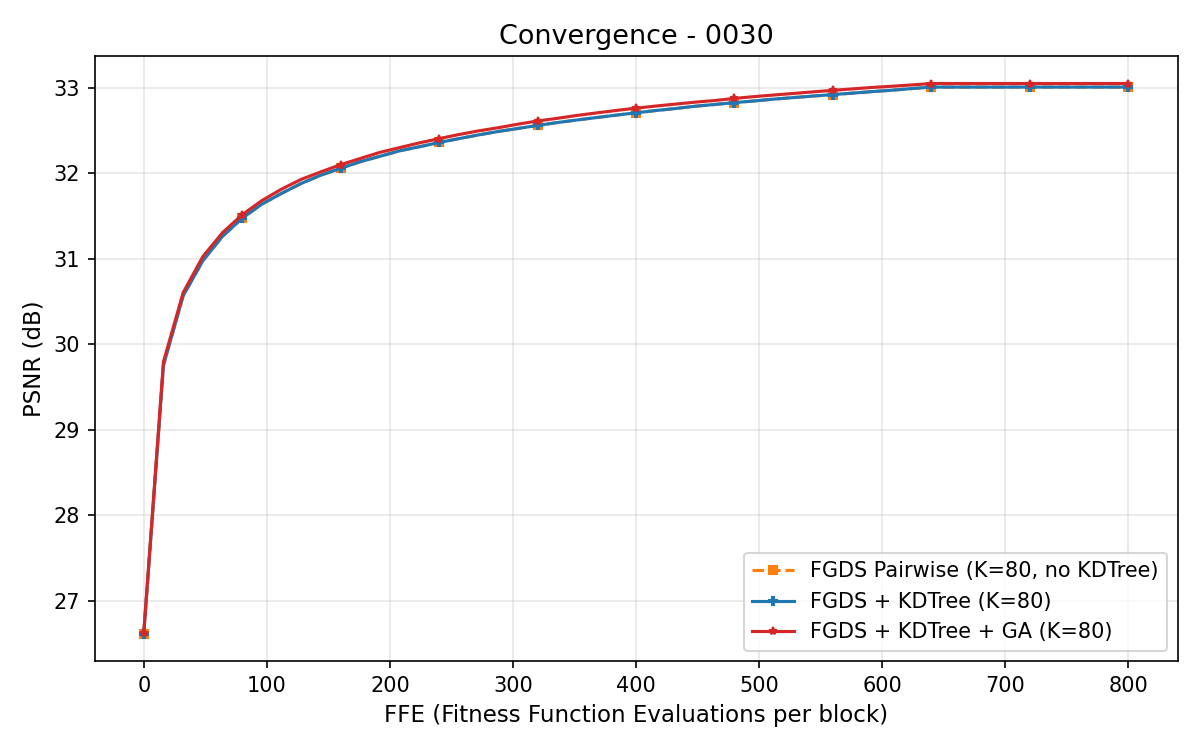
\includegraphics[width=\columnwidth]{images/convergence_0030.png}
    \caption{E2 convergence on image~0030. Pairwise and KD-Tree coincide exactly; KD-Tree+GA is marginally higher. All saturate at \mbox{$K\!\times\!8\!=\!640$}~FFEs.}
    \label{fig:conv_0030}
\end{figure}

\subsection{E3: Choosing the pool size \mbox{$K$}}

\begin{table}[t]
    \centering
    \caption{E3: \mbox{$K$}-sensitivity for KD-Tree FGDS, averaged over ten images. FFE is the effective per-block evaluation count under the 800-FFE protocol; rows with \mbox{$K\!\times\!8\le800$} are full exhaustive searches within the selected pool. MSE is encoder-side block-matching MSE.}
    \label{tab:k_sensitivity}
    \begin{tabular}{rlrrr}
        \toprule
        \mbox{$K$} & \textbf{FFE} & \textbf{PSNR (dB)} & \textbf{Enc. MSE} & \textbf{Total (s)} \\
        \midrule
        5          & 40           & 29.18              & 92.23             & 51.6               \\
        10         & 80           & 29.80              & 79.34             & 95.7               \\
        20         & 160          & 30.33              & 69.68             & 183.6              \\
        40         & 320          & 30.80              & 62.10             & 360.9              \\
        80         & 640          & 31.21              & 56.27             & 712.9              \\
        160        & 800 cap      & 31.33              & 54.65             & 884.7              \\
        \bottomrule
    \end{tabular}
\end{table}

Table~\ref{tab:k_sensitivity} shows diminishing returns. PSNR rises through \mbox{$K\!=\!80$} (31.21~dB), but \mbox{$K\!=\!160$} adds only +0.12~dB under the same 800-FFE cap while increasing time by about 1.24\mbox{$\times$}. Thus \mbox{$K=80$} is used as the quality--time default. Even \mbox{$K\!=\!40$} (30.80~dB) already exceeds every PSO baseline in Table~\ref{tab:results}.

\subsection{E4: Is it the features, or just a smaller pool?}

\begin{table}[t]
    \centering
    \caption{E4: feature-guided vs.\ random pool, both \mbox{$K\!=\!80$} exhaustive, identical FFEs. PSNR (dB).}
    \label{tab:random}
    \begin{tabular}{lrrrrr}
        \toprule
                  & 0002           & 0007           & 0029           & 0030           & 0032           \\
        \midrule
        Random-80 & 27.97          & 26.00          & 22.75          & 29.60          & 32.78          \\
        FGDS-80   & \textbf{30.35} & \textbf{27.95} & \textbf{25.81} & \textbf{32.69} & \textbf{35.89} \\
        \addlinespace[2pt]
                  & 0037           & 0043           & 0049           & 0051           & 0060           \\
        \midrule
        Random-80 & 31.16          & 26.96          & 29.01          & 27.15          & 26.21          \\
        FGDS-80   & \textbf{35.07} & \textbf{31.46} & \textbf{32.09} & \textbf{29.68} & \textbf{31.13} \\
        \bottomrule
    \end{tabular}
\end{table}

A natural objection is that any small exhaustive search might do well. E4 replaces the feature-guided pool with a same-size random pool (\mbox{$K\!=\!80$}) and keeps the exhaustive matcher identical. As Table~\ref{tab:random} and Fig.~\ref{fig:conv_random} show, FGDS beats the random pool on every image by 1.95--4.92~dB (average +3.25~dB; Wilcoxon \mbox{$p\!<\!0.01$}). The quality therefore comes from feature-guided \emph{selection}, not merely from using a smaller pool.

\begin{figure}[t]
    \centering
    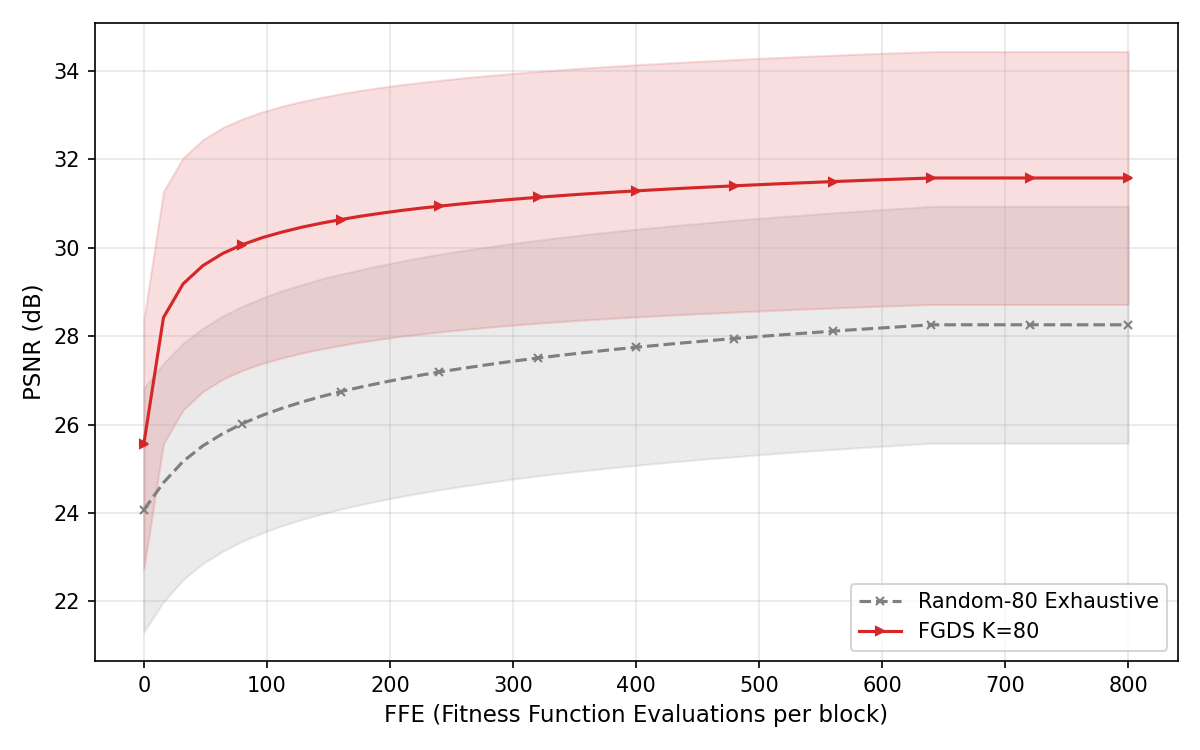
\includegraphics[width=\columnwidth]{images/convergence_average_random.png}
    \caption{E4 average convergence over ten images (\mbox{$\pm1\sigma$} bands). At equal FFEs, the feature-guided pool (red) consistently dominates a same-size random pool (gray) by approximately 3.25~dB across all search budgets.}
    \label{fig:conv_random}
\end{figure}

\subsection{Statistical significance}

\begin{table}[H]
    \centering
    \caption{Wilcoxon signed-rank tests (PSNR, one-sided, \mbox{$n=10$}).}
    \label{tab:wilcoxon}
    \small
    \setlength{\tabcolsep}{3pt}
    \begin{tabular}{lrrr}
        \toprule
        \textbf{Comparison}      & \textbf{Mean \mbox{$\Delta$}PSNR} & \mbox{$W^+$} & \mbox{$p$}     \\
        \midrule
        FGDS-40 vs.\ PSO         & +1.93                             & 55           & \mbox{$<0.01$} \\
        FGDS-40 vs.\ Memetic PSO & +1.65                             & 55           & \mbox{$<0.01$} \\
        FGDS-40 vs.\ FG-PSO      & +0.53                             & 55           & \mbox{$<0.01$} \\
        FGDS+GA-80 vs.\ PSO      & +2.39                             & 55           & \mbox{$<0.01$} \\
        FGDS+GA-80 vs.\ FGDS-80  & +0.05                             & 55           & \mbox{$<0.01$} \\
        FGDS-80 vs.\ Random-80   & +3.25                             & 55           & \mbox{$<0.01$} \\
        \bottomrule
    \end{tabular}
\end{table}

With \mbox{$n\!=\!10$} paired images and FGDS winning every pair, each test attains \mbox{$W^+\!=\!55$}, \mbox{$W^-\!=\!0$}, and exact one-sided \mbox{$p=1/2^{10}=0.00098$} (Table~\ref{tab:wilcoxon}). Thus the gains over PSO variants, the positive GA gain, and the random-pool advantage are all significant.

\begin{figure*}[!b]
    \centering
    \begin{minipage}{0.13\textwidth}
        \centering
        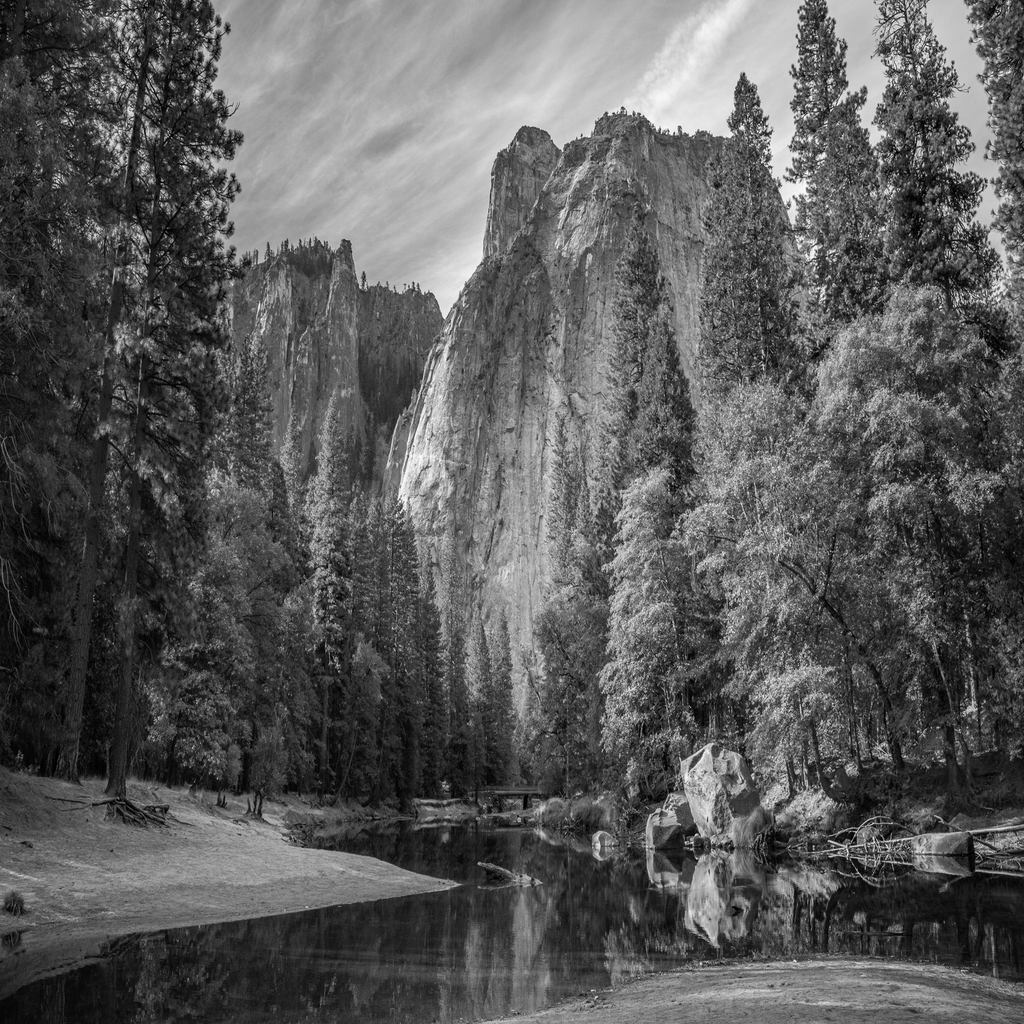
\includegraphics[width=\linewidth]{images/0007_original.png}\\[-2pt]
        {\scriptsize 0007 original}
    \end{minipage}
    \hspace{0.006\textwidth}
    \begin{minipage}{0.13\textwidth}
        \centering
        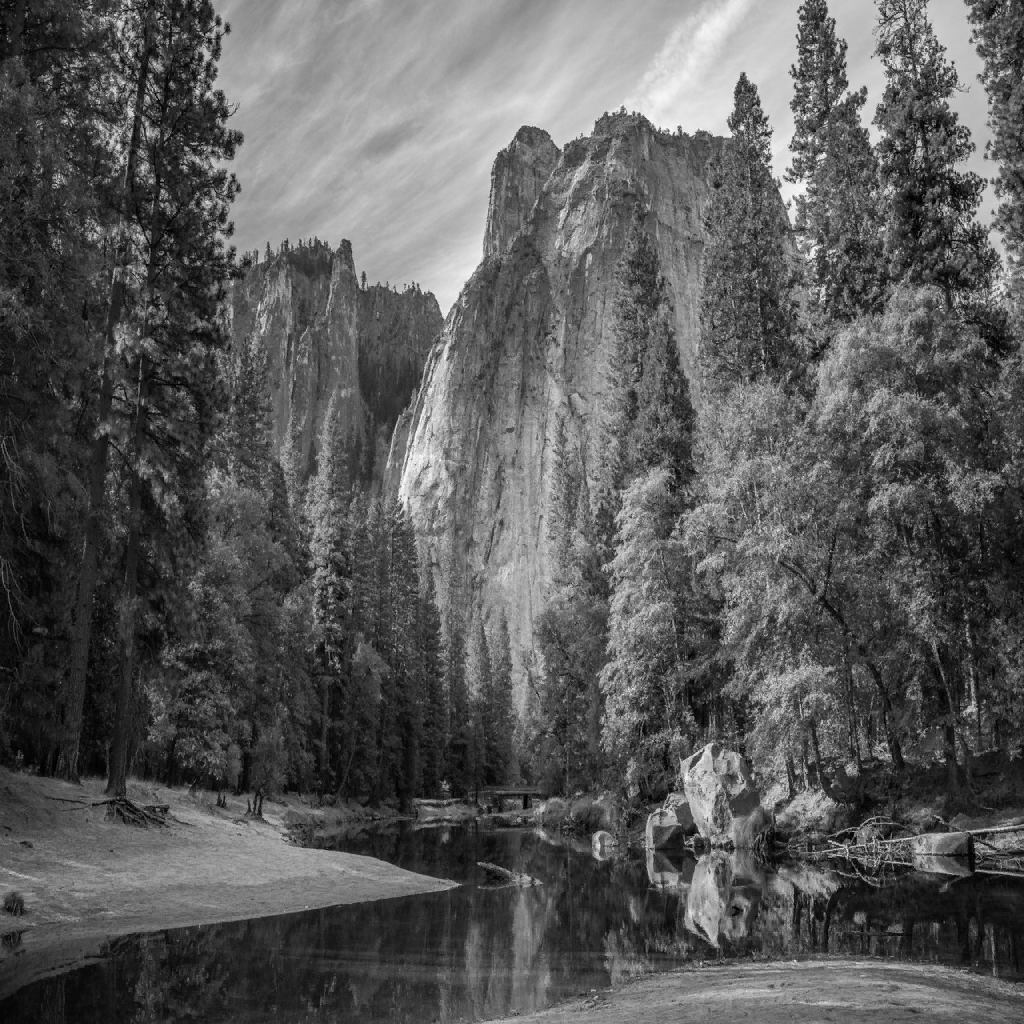
\includegraphics[width=\linewidth]{images/0007_fgds_ga_reconstructed.png}\\[-2pt]
        {\scriptsize 0007 FGDS+GA}
    \end{minipage}
    \hspace{0.012\textwidth}
    \begin{minipage}{0.13\textwidth}
        \centering
        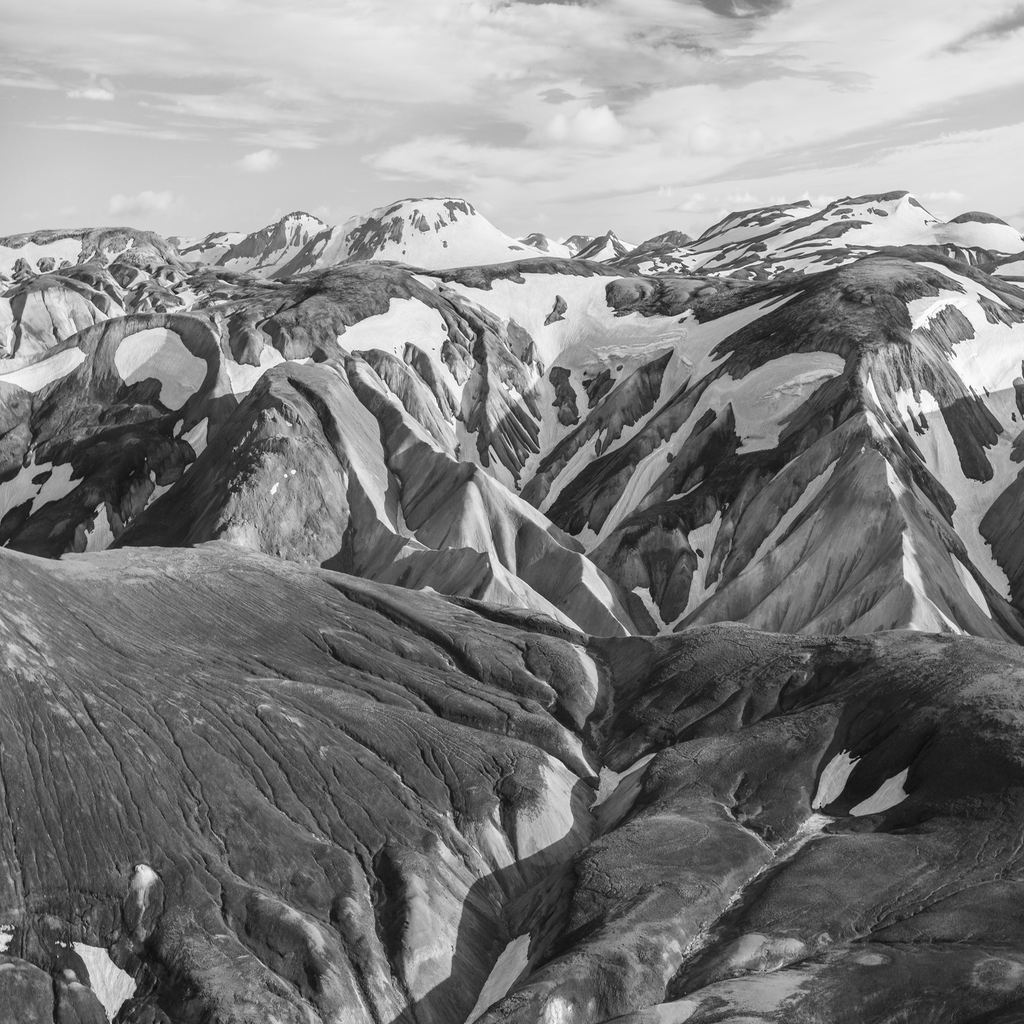
\includegraphics[width=\linewidth]{images/0030_original.png}\\[-2pt]
        {\scriptsize 0030 original}
    \end{minipage}
    \hspace{0.006\textwidth}
    \begin{minipage}{0.13\textwidth}
        \centering
        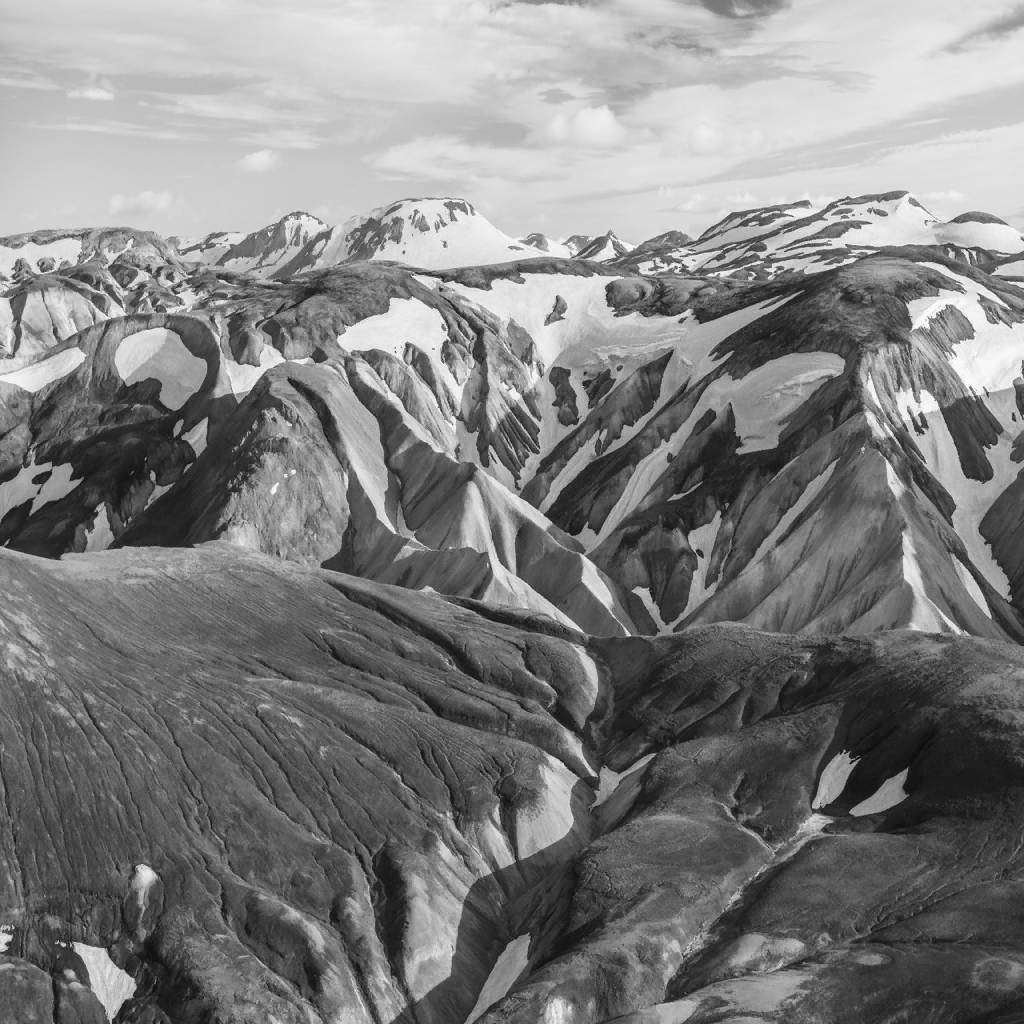
\includegraphics[width=\linewidth]{images/0030_fgds_ga_reconstructed.png}\\[-2pt]
        {\scriptsize 0030 FGDS+GA}
    \end{minipage}
    \hspace{0.012\textwidth}
    \begin{minipage}{0.13\textwidth}
        \centering
        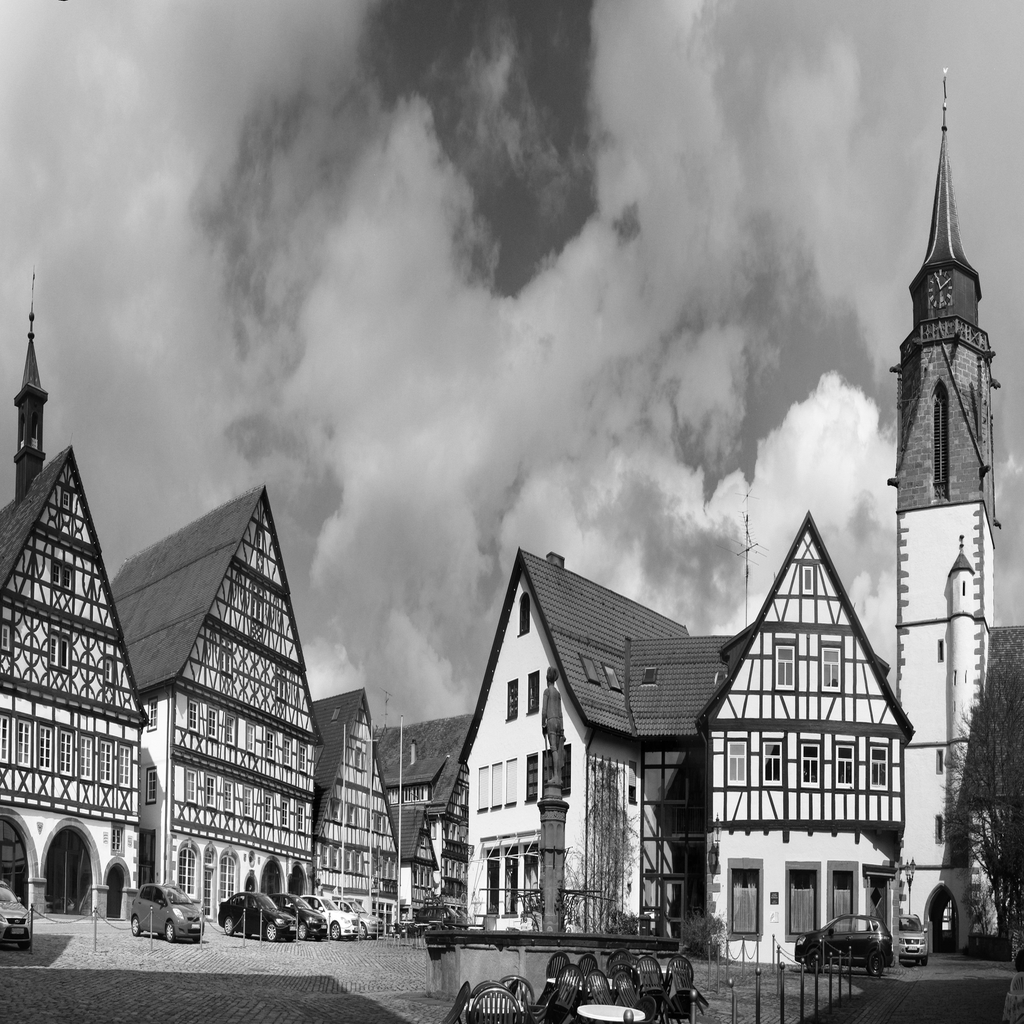
\includegraphics[width=\linewidth]{images/0060_original.png}\\[-2pt]
        {\scriptsize 0060 original}
    \end{minipage}
    \hspace{0.006\textwidth}
    \begin{minipage}{0.13\textwidth}
        \centering
        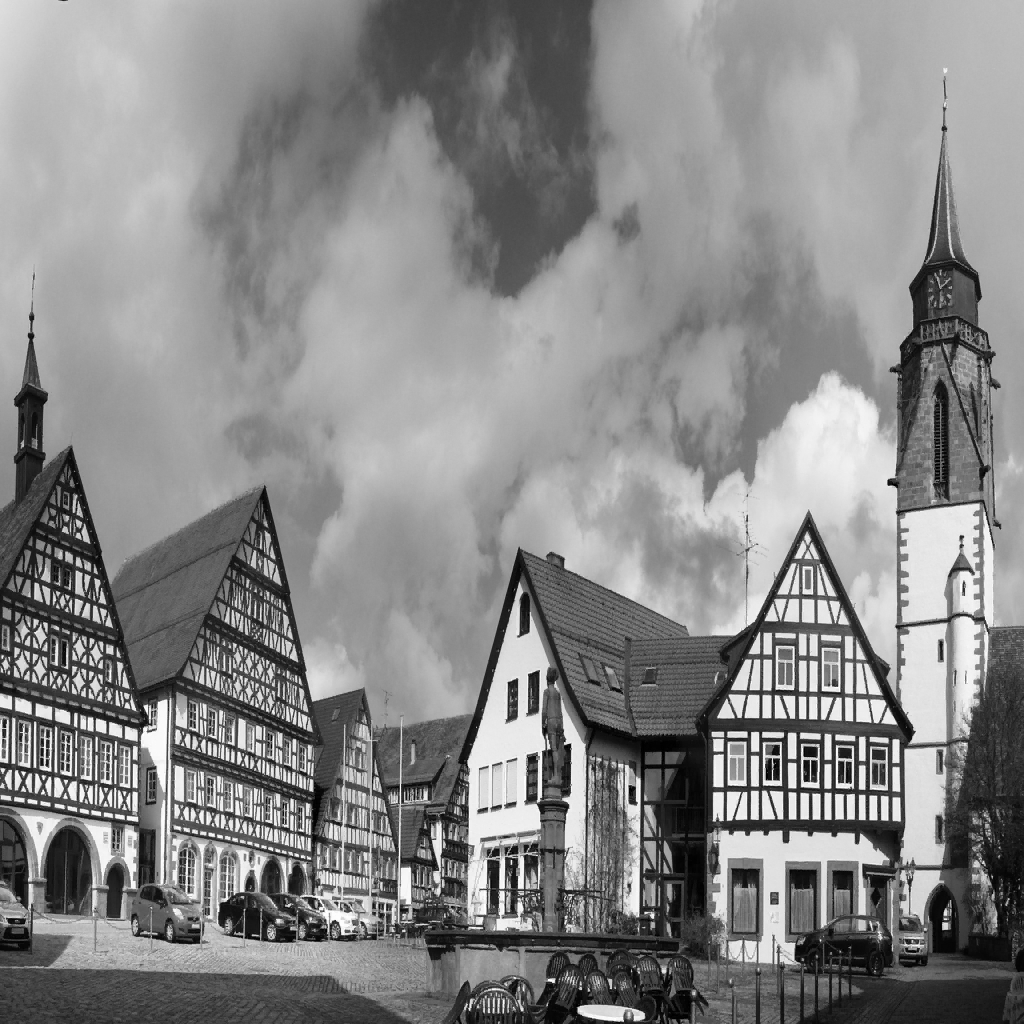
\includegraphics[width=\linewidth]{images/0060_fgds_ga_reconstructed.png}\\[-2pt]
        {\scriptsize 0060 FGDS+GA}
    \end{minipage}
    \caption{Original images and FGDS+GA reconstructions at \mbox{$K=80$}.}
    \label{fig:visual}
\end{figure*}

%% ================================================================
\section{Discussion and Limitations}
%% ================================================================

The results should be read as evidence for search-space construction, not as a codec-level state-of-the-art claim. The GA weighting gives only a small PSNR gain (+0.05~dB on average), while the main improvement comes from feature-guided selection. The study is limited to grayscale images, fixed block sizes, a fixed code structure, and PSNR measured before coefficient quantization; color images, adaptive partitions, other bit rates, and bitstream-decoded PSNR remain future work.


%% ================================================================
\section{Conclusion}
%% ================================================================

This work shows that high-resolution FIC is limited less by the optimizer than by candidate-space quality. FGDS shifts the heuristic from block \emph{matching} to block \emph{selection} using isometry-robust features, KD-Tree retrieval, and offline GA-learned weights. It improves PSNR over PSO by 1.93~dB at \mbox{$K\!=\!40$} and 2.39~dB at \mbox{$K\!=\!80$} (with GA), with all gains significant at \mbox{$p<0.01$}. The random-pool control confirms that the improvement comes from feature-guided selection rather than search-space reduction alone.

\bibliographystyle{IEEEtran}
\IEEEtriggeratref{19}
\bibliography{references}

\vspace{12pt}

\end{document}
